\subsubsection{ Radar Simulator Use Cases}
\begin{figure}[h]
\caption{Radar simulator Use Case Diagram}
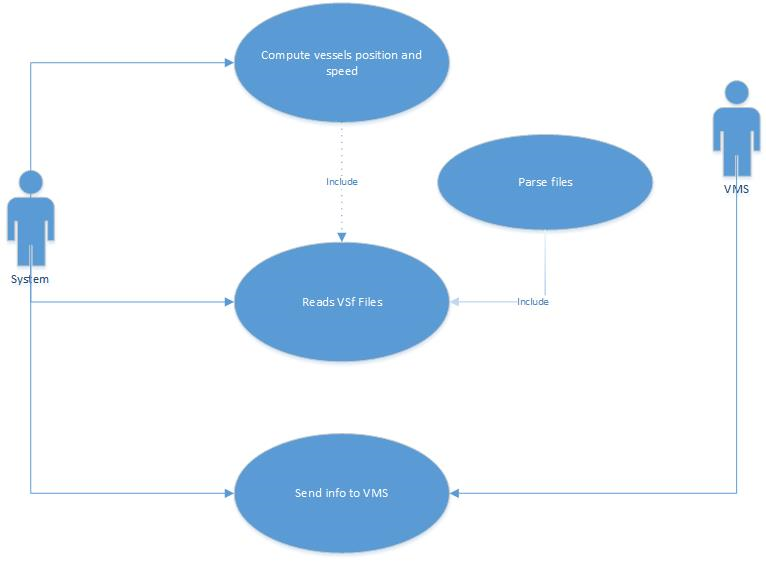
\includegraphics[width=0.8\textwidth]{usecasediagram}
\end{figure}

\noindent
{\bf Name}\\
Radar simulation -Normal Running process

\noindent
{\bf Actors}\\
Vessel monitoring system ,java system

\noindent
{\bf Goals}\\
to send valid vessels information to the vms 

\noindent
{\bf Preconditions }\\
a vsf  file is created and place in the required locations 
the file has information on different vessels

\noindent
{\bf Summary }\\
the radar simulator will read the location of different type of vessel in a range of 5000 meters,
computes the location and directions of each vessels, 
sends the different informations to the vessel monitoring system ,updates every time the vessels  
change position or location

\noindent
{\bf steps }\\ 
\begin{enumerate}
\item  read  the vsf file  by the systems 
\item validate the vsf files by cheking that there is information on the file 
\item read each line of the file 
\item disregard any comments that is find in the file.
\item calculates the speed,location directions
\item send the different information to the VMS
\item repeat step three until quit by the system
\end{enumerate} 

\noindent
{\bf Name}\\
Radar simulation -File not valid 

\noindent
{\bf Actors}\\
java system 

\noindent
{\bf Goals}\\
to open tht vsf files and make sure that its valid 

\noindent
{\bf Preconditions }\\
a vsf  file is created and place in the required locations 


\noindent
{\bf Summary }\\
the radar simulator will read the location of different type of vessel in a range of 5000 meters,
computes the location and directions of each vessels, 
sends the different informations to the vessel monitoring system ,updates every time the vessels  
change position or location

\noindent
{\bf steps }\\
\begin{enumerate}
\item open the vsf files, 
\item tries to see if its possible to open the file 
\item stop the rader simulator and send handle file not found exception 
\end{enumerate} 
